\documentclass[sigconf, nonacm]{acmart}
\settopmatter{printfolios=true}
\settopmatter{printacmref=false}
%% PACKAGES
\usepackage{graphicx}
\usepackage{hyperref}
\usepackage{cleveref}
\usepackage{subcaption}
\usepackage{natbib}
\usepackage{mathtools}
\usepackage{xcolor}

%% COLORS
\definecolor{darkgreen}{rgb}{0,0.8,0}

%% TITLES
\title{ALTEGRAD Challenge 2024 on Molecules and NLP: contrastive learning applied to retrieval systems of chemical compounds}

%% AUTHORS
\author{Balthazar Neveu}
\affiliation{%
  \institution{ENS Paris-Saclay}
  \city{Saclay}
  \country{France}
}
\email{balthazar.neveu@ens-paris-saclay.fr}

\author{Léa Khalil}
\affiliation{%
  \institution{Ecole Polytechnique}
  \city{Palaiseau}
  \country{France}
}
\email{leakhalil@yahoo.fr}

\author{Basile Terver}
\affiliation{%
  \institution{Ecole Polytechnique}
  \city{Palaiseau}
  \country{France}
}
\email{terverbasile@gmail.com}


%% MAIN DOCUMENT
\begin{document}

  %% KEYWORDS
  \keywords{contrastive learning, graph neural networks, large language models}

  %% Teaser figure
% \begin{figure*}[ht]
  \begin{teaserfigure}
    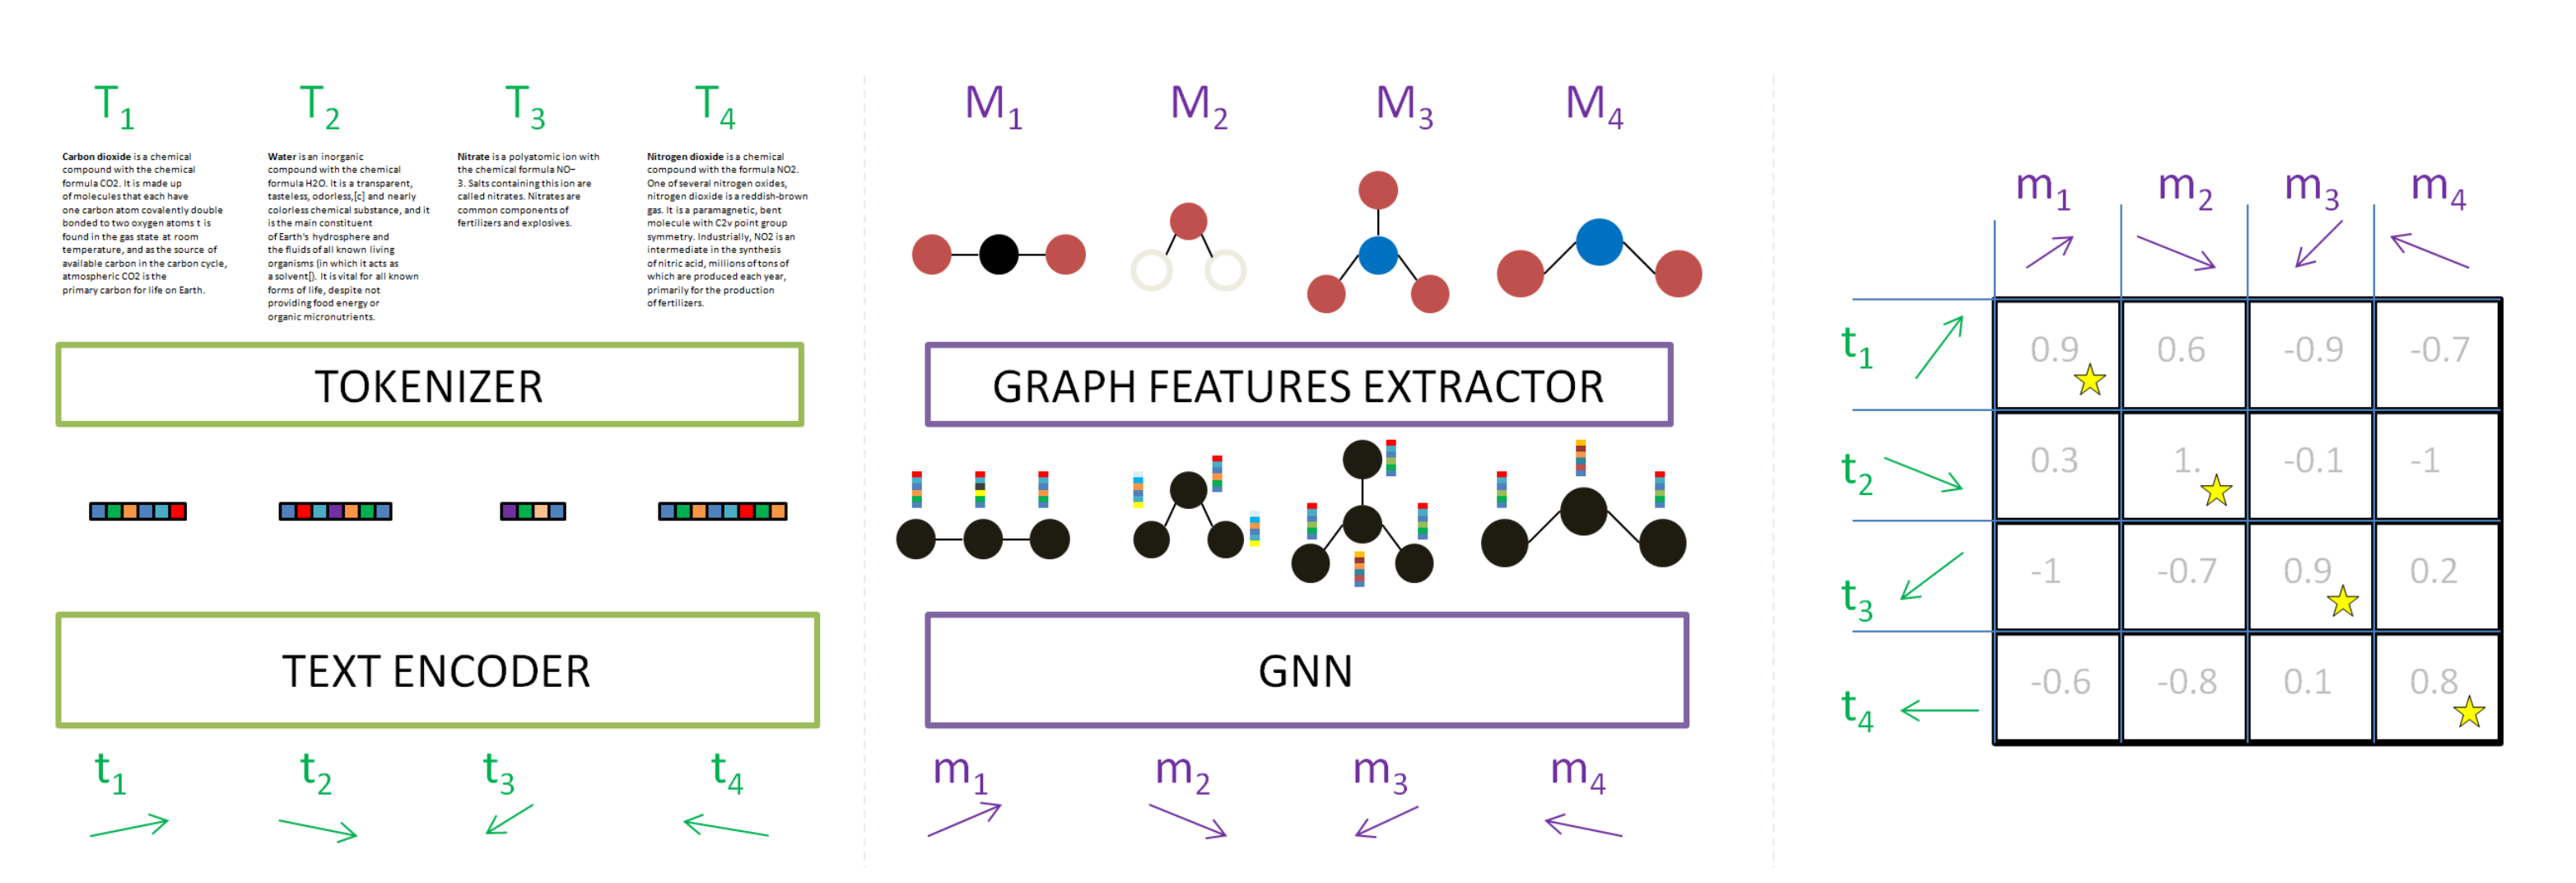
\includegraphics[width=0.9\textwidth]{figures/mol_text_overview.PNG}
    \centering
    \caption{Our system matches a text description with the most relevant molecules. On the left side, text descriptions $T_{i}$ are tokenized and transformed into a numerical representations (embeddings) $t_{i}$ using a large language model. In the center, molecules $M_{j}$ are represented using graphs where each node is a molecular structure (not just an atom) attached with its vector representation. Graphs are processed by a graph neural network to create embeddings $m_{j}$. On the right side, pairwise similarity matrix between text and molecule allows finding the best matches (ranking) and is also the central mathematical object used to train the system (contrastive learning means maximizing $\vec{t_{i}}.\vec{m_{i}}$ and minimizing $\vec{t_{i}}.\vec{m_{j}}$  $\forall j \neq i$).
    }
    \label{fig:original_pipeline}
\end{teaserfigure}
% \end{figure*}

  %% TITLE
\maketitle


  %% ABSTRACT

  %% CONTENT
  \section{Introduction}
\label{sec:intro}
Text-2-Mol \cite{text2mol} introduced the groundings of the problem of pairing a text description with the corresponding molecule.
Their contribution also cam with a dataset made of 33k which is always appreciated among the research community.
Here we're using this dataset and the problem is restricted to using this data solely.
We're leveraging the language understanding contained in pretrained Large Language Models (LLM) to create embeddings for text descriptions.
We at least start with models that have good understanding of the English language. The whole point is to transfer this knowledge to the chemical domain to be able to understand molecule structure from a description.
Our code is available on ~\href{https://github.com/balthazarneveu/molecule-retrieval-u sing-nlp}{GitHub}.



  \section{Context}
\label{sec:Context}


\subsection{Dataset}
\label{sec:sota}

\color{red}TODO - Describe dataset in depth and challenge \color{black}


\subsection{State of the art}
\label{sec:sota}

\color{red}TODO - State of the art - Text2mol, CLIP, MolICLR augmentations=Contrastive learning for molecules only\color{black}



\subsubsection{BERT: our base LLM}
\label{sec:bert}
\color{red}TODO - Describe BERT and Distil BERT and SciBERT\color{black}



\subsubsection{GCN: graph convolution networks}
\label{sec:GCN}
\color{red}TODO - Quickly recall Kipf and Welling + using Pytorch geometry (sparse graphs?)\color{black}
  \section{Implementation Strategy}
\label{sec:remplementation}
\subsection*{Methodology}
\label{sec:methodology}
As this work was to  be done in group, we have to develop a framework so everyone could work and share their code independently.
\begin{itemize}
    \item Heterogeneous environments: several operating systems (linux, windows, macOS), various platforms (local laptop training, Kaggle Kernels notebook, remote machines at Ecole Polytechnique). On every platform, data has to be acessible and experiments results have to be stored in a way they can be retrieved. We used the Kaggle dataset feature to  host the raw dataset aswell as the preprocessed data.
    \item Privacy: as not sharing code was among the rules of the challenge, our source code remained private on GitHub (\textit{which made cloning operations even trickier when using Kaggle kernels}).
    \item Reproducibility: all our experiments are reproducible (source code tracking under git, local and cloud storage of experiments results using ~\href{https://wandb.ai/molecule-nlp-altegrad-23/molecule-nlp}{Weights and biases}).
\end{itemize}
An experiment is defined by a unique identifier and the instanciation of a model (tokenization method, architecture of the LLM and GNN), the configuration of an  optimizer and training hyper parameters. At inference time, we're using this unique identifier so we can safely instantiate a network and reload the weights (\textit{trained model are by construction compatible with inference. This avoids the risk of having a `.pth` weight file without knowning which architecture to use to reload it.}).
We wrote a framework which takes and solves all these constraints at once and allows to focus on training models.


\subsection*{Training conditions}
\label{sec:training conditions}
To setup the training loop, we started on a single NVIDIA GeForce RTX 2080 GPU with 6Gb of RAM. This was enough to make sure we could train, track and monitor progress of all our experiments.


\begin{table*}[ht]
    \centering
    \begin{tabular}{lcccc}
    \hline
    \textbf{Feature} & \textbf{Nvidia T500} & \textbf{Nvidia RTX 2060} & \textbf{Nvidia K100} & \textbf{Nvidia A4000} \\ \hline
    Location            & local laptop           & local laptop  & Kaggle  & Ecole Polytechnique  \\
    Access & direct & direct & Kaggle Kernels & SSH \\
    Dataset access & local SSD & local SSD & Kaggle dataset & remote download + SSD drives\\ 
    Memory           & 4 GB                        & 6 GB                           & 16 GB                          & 24 GB                          \\
    \hline
    \end{tabular}
    \caption{Comparison of the GPUs which were used during training}
    \label{table:gpu_comparison}
\end{table*}


\pagebreak

\subsection*{Preliminary study}
\label{sec:preliminary study}

\begin{table*}[h]
    \centering
    \begin{tabular}{|c|c|c|c|c|}
    \hline
    \textbf{Experiment ID} & \textbf{Model Size} & \textbf{LLM} & \textbf{GNN} & \textbf{LRAP} \\ \hline
    101         & 593k                & Frozen Distill-Bert           & Base 3 layer GCN       & 18.7\%      \\ \hline
    106         & 964k                & Frozen Distill-Bert + Adapter & Base 3 layer GCN       & 26.8\%      \\ \hline
    114         & 2.125M              & Frozen Distill-Bert + Adapter & Big 5 layer GCN        & 31.6\%      \\ \hline
    112         & 964k                & Frozen Sci-Bert + Adapter     & Base 3 layer GCN       & 36.7\%      \\ \hline
    113         & 2.125M              & Frozen Sci-Bert + Adapter     & Big 5 layer GCN        & 39.8\%      \\ \hline
    65          & 66.9M               & Trainable Bert                & Base 3 layer GCN       & 63.5\%      \\ \hline
    400         & 110M                & Trainable Sci-Bert            & Base 3 layer GCN       & 66\%        \\ \hline
    \end{tabular}
    \caption{Base Models Specifications and Performances}
    \label{tab:preliminary_study_metrics}
\end{table*}


We start with a few toy experiments to see which architecture factors are most promising (initial hope is that the performances will scale accordingly when we add all extra machine learning tricks).
\textbf{Frozen LLM weights}: We first started with by simple models based on the base GCN (3 graph convolution layers followed by a global pooling layer and 2 layers MLP). Instead of fine tuning all parameters of the LLM, we first started by freezing the LLM parameters. Although simple, this idea intuivitely has many advantages for traing:
\begin{itemize}
    \item We discard the huge memory cost of training a LLM (memory issues not only come from storing the weigths on the GPU but all the optimizers variables during backpropagation). The idea could have been pushed further by pre-computing the text embeddings and storing them on disk. 
    \item Intuivitely, freezing the LLM parameters should make the training more stable as the LLM embeddings acts as a kind of anchor that the GNN shall match.
\end{itemize}
Unfortunately, training achieves low accuracy although the number of parameters to train is lightweight. We added an "adapter" module which is simply a MLP which will adapt by projecting the text representations into a more adapted space which can match with the graph.
\textbf{Influence of the graph neural network size}: We pursued our explorations to see the impact of the GNN size. The \textbf{big GCN} (5 graph convolution layers with 2 residual connection) is more complex and has more parameters to train. We can see that the accuracy is improved by increasing the GCN size. 
\begin{itemize}
    \item Using frozen Distil-BERT: from experiment 106 (base GCN $\text{LRAP}=26.8\%$) to 114 - (big GCN $\text{LRAP}=31.6\%$)
    \item Using frozen SciBERT: from experiment 102 (base GCN $\text{LRAP}=36.7\%$) to 113 - (big GCN $\text{LRAP}=39.8\%$)
\end{itemize}


\textbf{Influence of the pretrained language model}: We also browsed Hugging Face to find models that could be dedicated to scientific-specific language processing. We foud the Sci-Bert\cite{scibert} model and could use it as a drop-in replacement for the Distil-Bert baseline model. Improvements were two-fold when changing the pretrained LLM during this preliminary study: a tokenizer dedicated to a scientific corpus seems by nature a natural choice for scientific words...here atoms and molecule names not being too frequent in common language. The Sci-Bert model may also have reasoning capabilities closer to science and chemistry reactions. This was translated by a improvement in performances. Increasing the GNN size improves accuracy.
\begin{itemize}
    \item Using the Base GCN : from experiment 106 Distil-BERT ($\text{LRAP}=26.8\%$) to experiment 112 - SciBert ($\text{LRAP}=36.7\%$).
    \item Using the Big-GCN: from experiment 114 Distil-BERT ($\text{LRAP}=31.6\%$) to experiment 113 - SciBert ($\text{LRAP}=39.8\%$).
\end{itemize}
The capacity of the network (same number of parameters) being fixed between these two experiments, it proves that the SciBERT tokenization and pretraining is definitely more suited for our task. We'd hope that this $seq 8\%$ LRAP improvement would be translated when training a fully trainable LLM.

Unfortunately we later conducted larger experiments with fully trainable LLM (starting from the pretrained weights) and the performances differences were not as good as expected. Using the Base GCN : from experiment 65 Distil-BERT ($\text{LRAP}=63.5\%$) to experiment 400 - SciBert ($\text{LRAP}=66\%$), there's not that $seq 8\%$ LRAP improvement that we had seen earler. Furthermore, it's hard to tell whether the 2.5\% improvement is due to the SciBert model pretraining being more suited for our task or the fact that the model has nearly twice as many trainable parameters than the Distil-BERT. 

This preliminary study gave us guidance that using a larger GCN and using SciBERT pretrained weights and tokenizer were good trends to follow to try improving our results. The pitfall is that fine tuning SciBERT comes with a bigger memory footprint than Distil-BERT which requires diminishing batch sizes for a fixed GPU (and as stated in the CLIP paper, large batch size seems to be one key factor of the success of contrastive learning). Experiments 65 and 400 have been cautiousy trained with batches of size 32 and same hyperparameters to get comparable results: 
\begin{itemize}
    \item the SciBERT experiment 400 was only possible using a NVIDIA RTX A4000 with 24Gb of RAM \item the Distil-BERT experiment 65 was possible on a NVIDIA Tesla T100 with 16Gb of RAM (Kaggle Kernels notebook).
\end{itemize}



\begin{figure*}[ht]
    \centering
    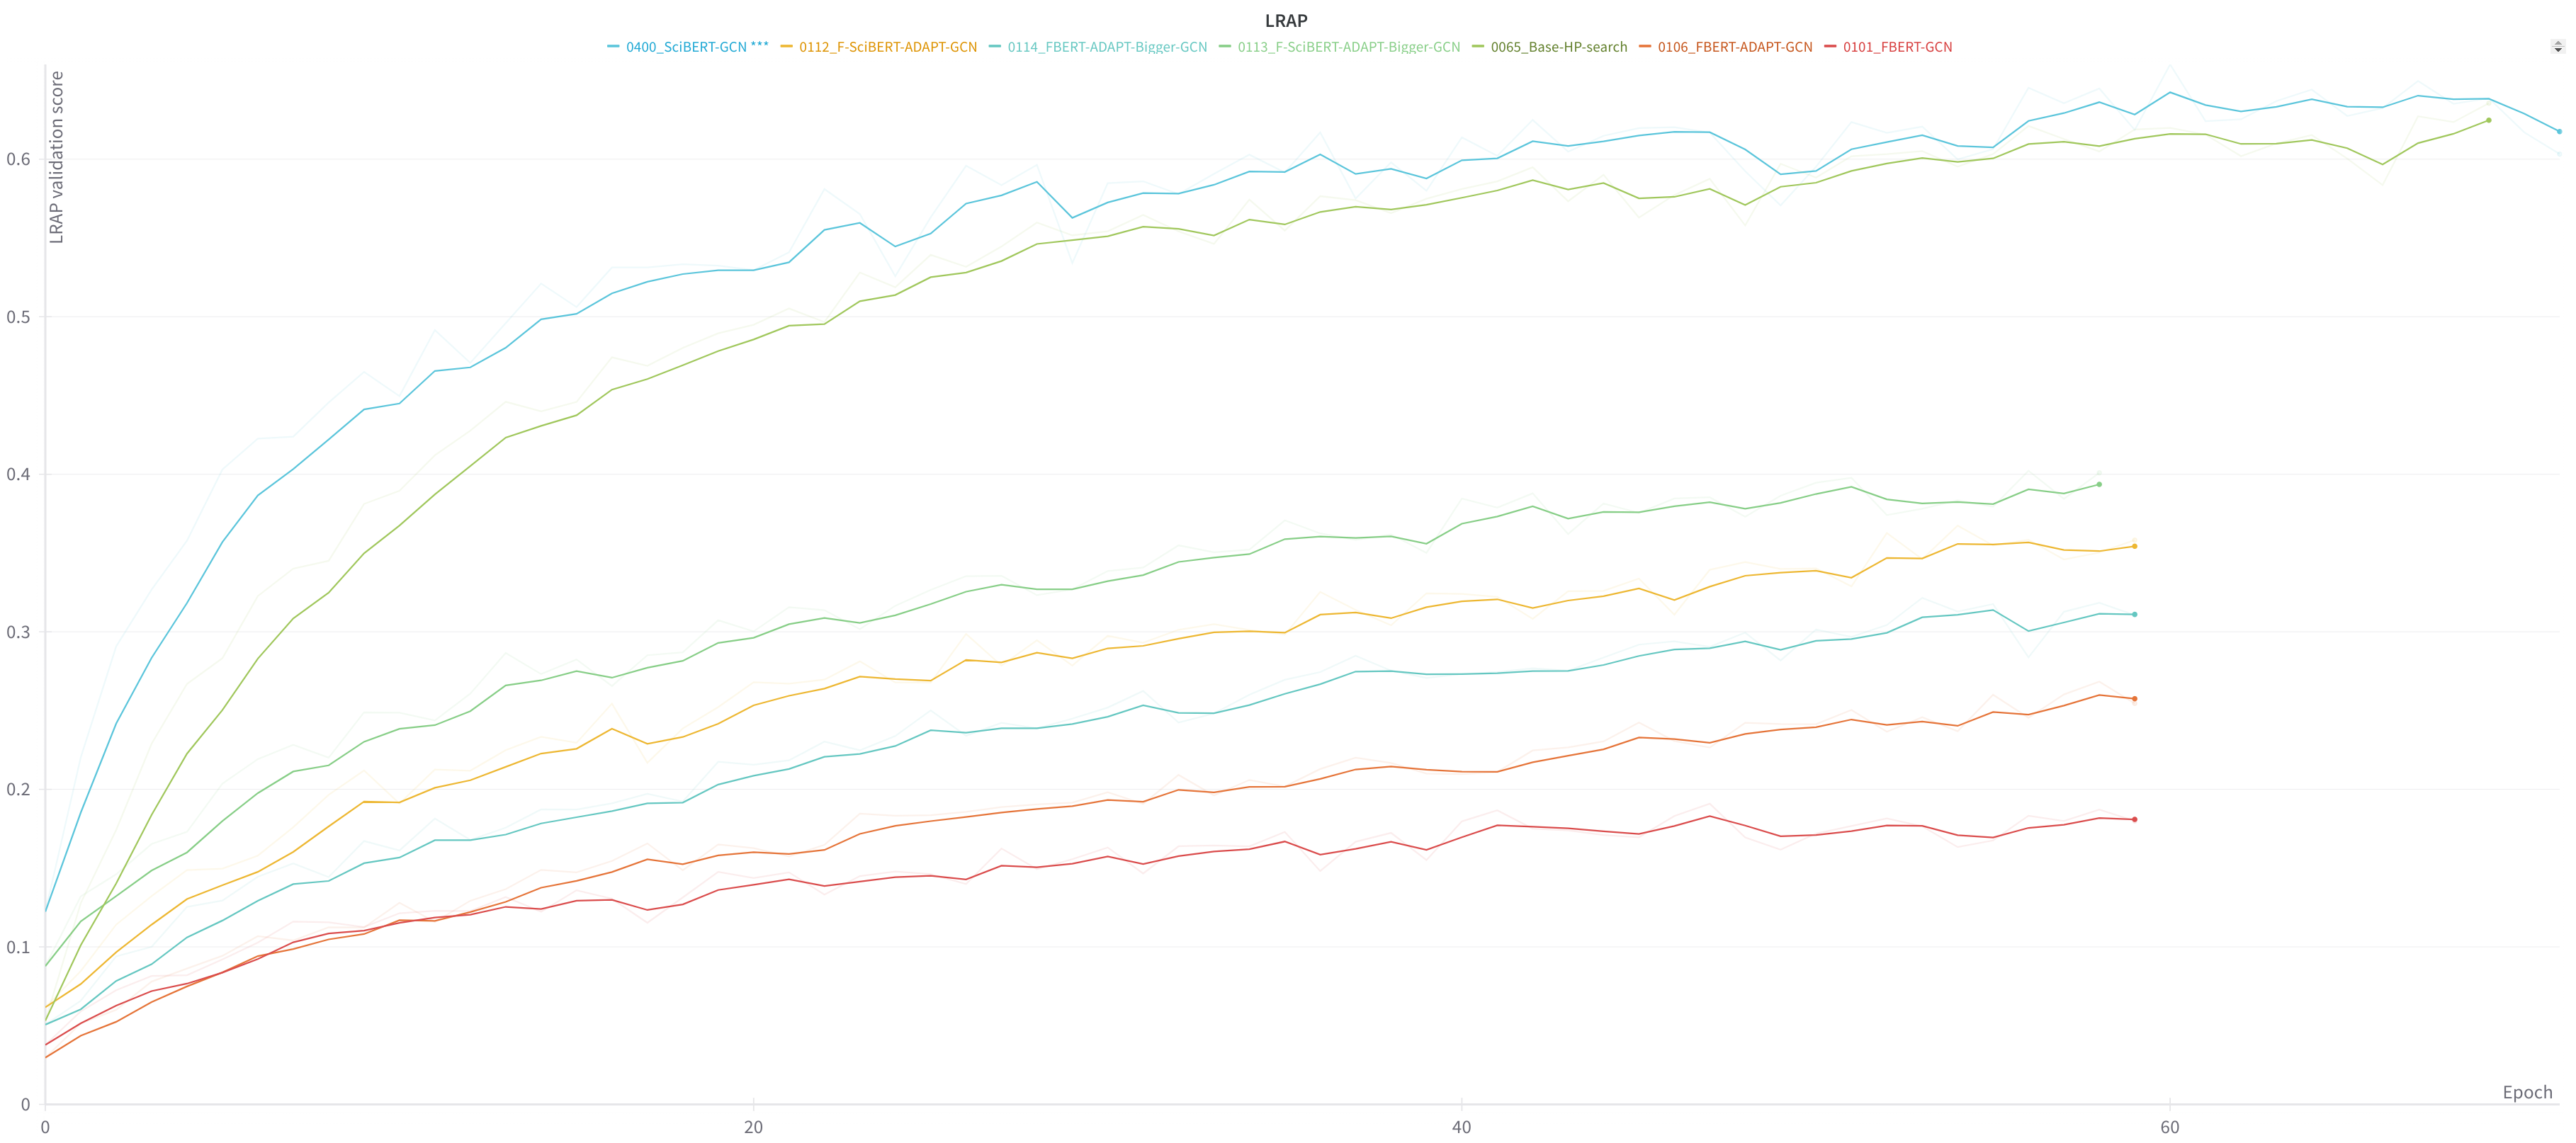
\includegraphics[width=1.\textwidth]{figures/preliminary_study.png}
    \caption{Training curves for the preliminary study.}
    \label{fig:preliminary_study_curves}
\end{figure*}


  \section{Discussion on the Paper}
\label{sec:discussion}
Discussion
  \section{Conclusion}
\label{sec:conclusion}

In conclusion...


  \newpage
  %% BIBLIOGRAPHY
  \bibliographystyle{ACM-Reference-Format}
  \bibliography{references}
  \newpage
  %% APPENDIX
  \appendix
  \section{Appendix}
Appendix
  


\clearpage
\section{Appendix: Training framework}
\label{sec:training_fwk}
This section describes the work which was done at software level which is definitely not a part that can be neglected when working in group on such a complex machine learning project (a lot of heavy computation power required, long training times for limited chances for improvements).  We describe the constraints we had to face and the solutions we found to overcome them. We trained nearly a hundred experiments which requires good organization and a way to track and monitor everything.
We came out with a convenient solution which allows respecting all the project constraints and allowed us to focus on the machine learning part of the project.

\subsection*{Constraints statement}
\label{sec:Constraints}
As this work was to be done in group, we had to develop a framework to guarantee that everyone could work and share their code independently.
\begin{itemize}
    \item Heterogeneous environments: several operating systems (linux, windows, macOS), various platforms (local laptop training, Kaggle Kernels notebook, remote machines at Ecole Polytechnique). On every platform, data has to be acessible and experiments results have to be stored in a way they can be retrieved. We used the Kaggle dataset feature to  host the raw dataset as well as the preprocessed data.
    \item Privacy: as not sharing code was among the rules of the challenge, our source code remained private on GitHub (\textit{which made cloning operations even trickier when using Kaggle kernels}).
    \item Reproducibility: all our experiments are reproducible (source code tracking under git, local and cloud storage of experiments results using ~\href{https://wandb.ai/molecule-nlp-altegrad-23/molecule-nlp}{Weights and biases}).
    \item Cost: project total budget limit to 50euros. \textit{Google Colab would not have met this requirement considering the amount of experiments we did and the long training times}.
\end{itemize}


We wrote a framework which takes and solves all these constraints at once and allows to focus on training models.

\subsection*{Definition of an experiment}
An experiment is defined by a unique identifier and the instantiation of a model (tokenization method, architecture of the LLM and GNN), the configuration of an  optimizer and training hyper parameters. At inference time, we're using this unique identifier so we can safely instantiate a network and reload the weights (\textit{trained model are by construction compatible with inference. This avoids the risk of having a `.pth` weight file without knowing which architecture to use to reload it.}).
Launching the training of an experiment goes seamlessly with the following command line, below is the example for experiment 620:
\begin{verbatim}
    python train.py -e 620
\end{verbatim}

The same exact training can be ran directly on Kaggle using their API.
\begin{verbatim}
    python remote_training.py -e 620 -p -nb mol-nlp
\end{verbatim}
Finally, the evaluation mechanism generates the submission csv file and the right Kaggle API command line which can be used to submit to the hosted challenge (with a message which allows to know exactly which experiment was submitted in which conditions).

\begin{verbatim}
python evaluation.py -e 620
\end{verbatim}

\begin{figure}
    \centering
    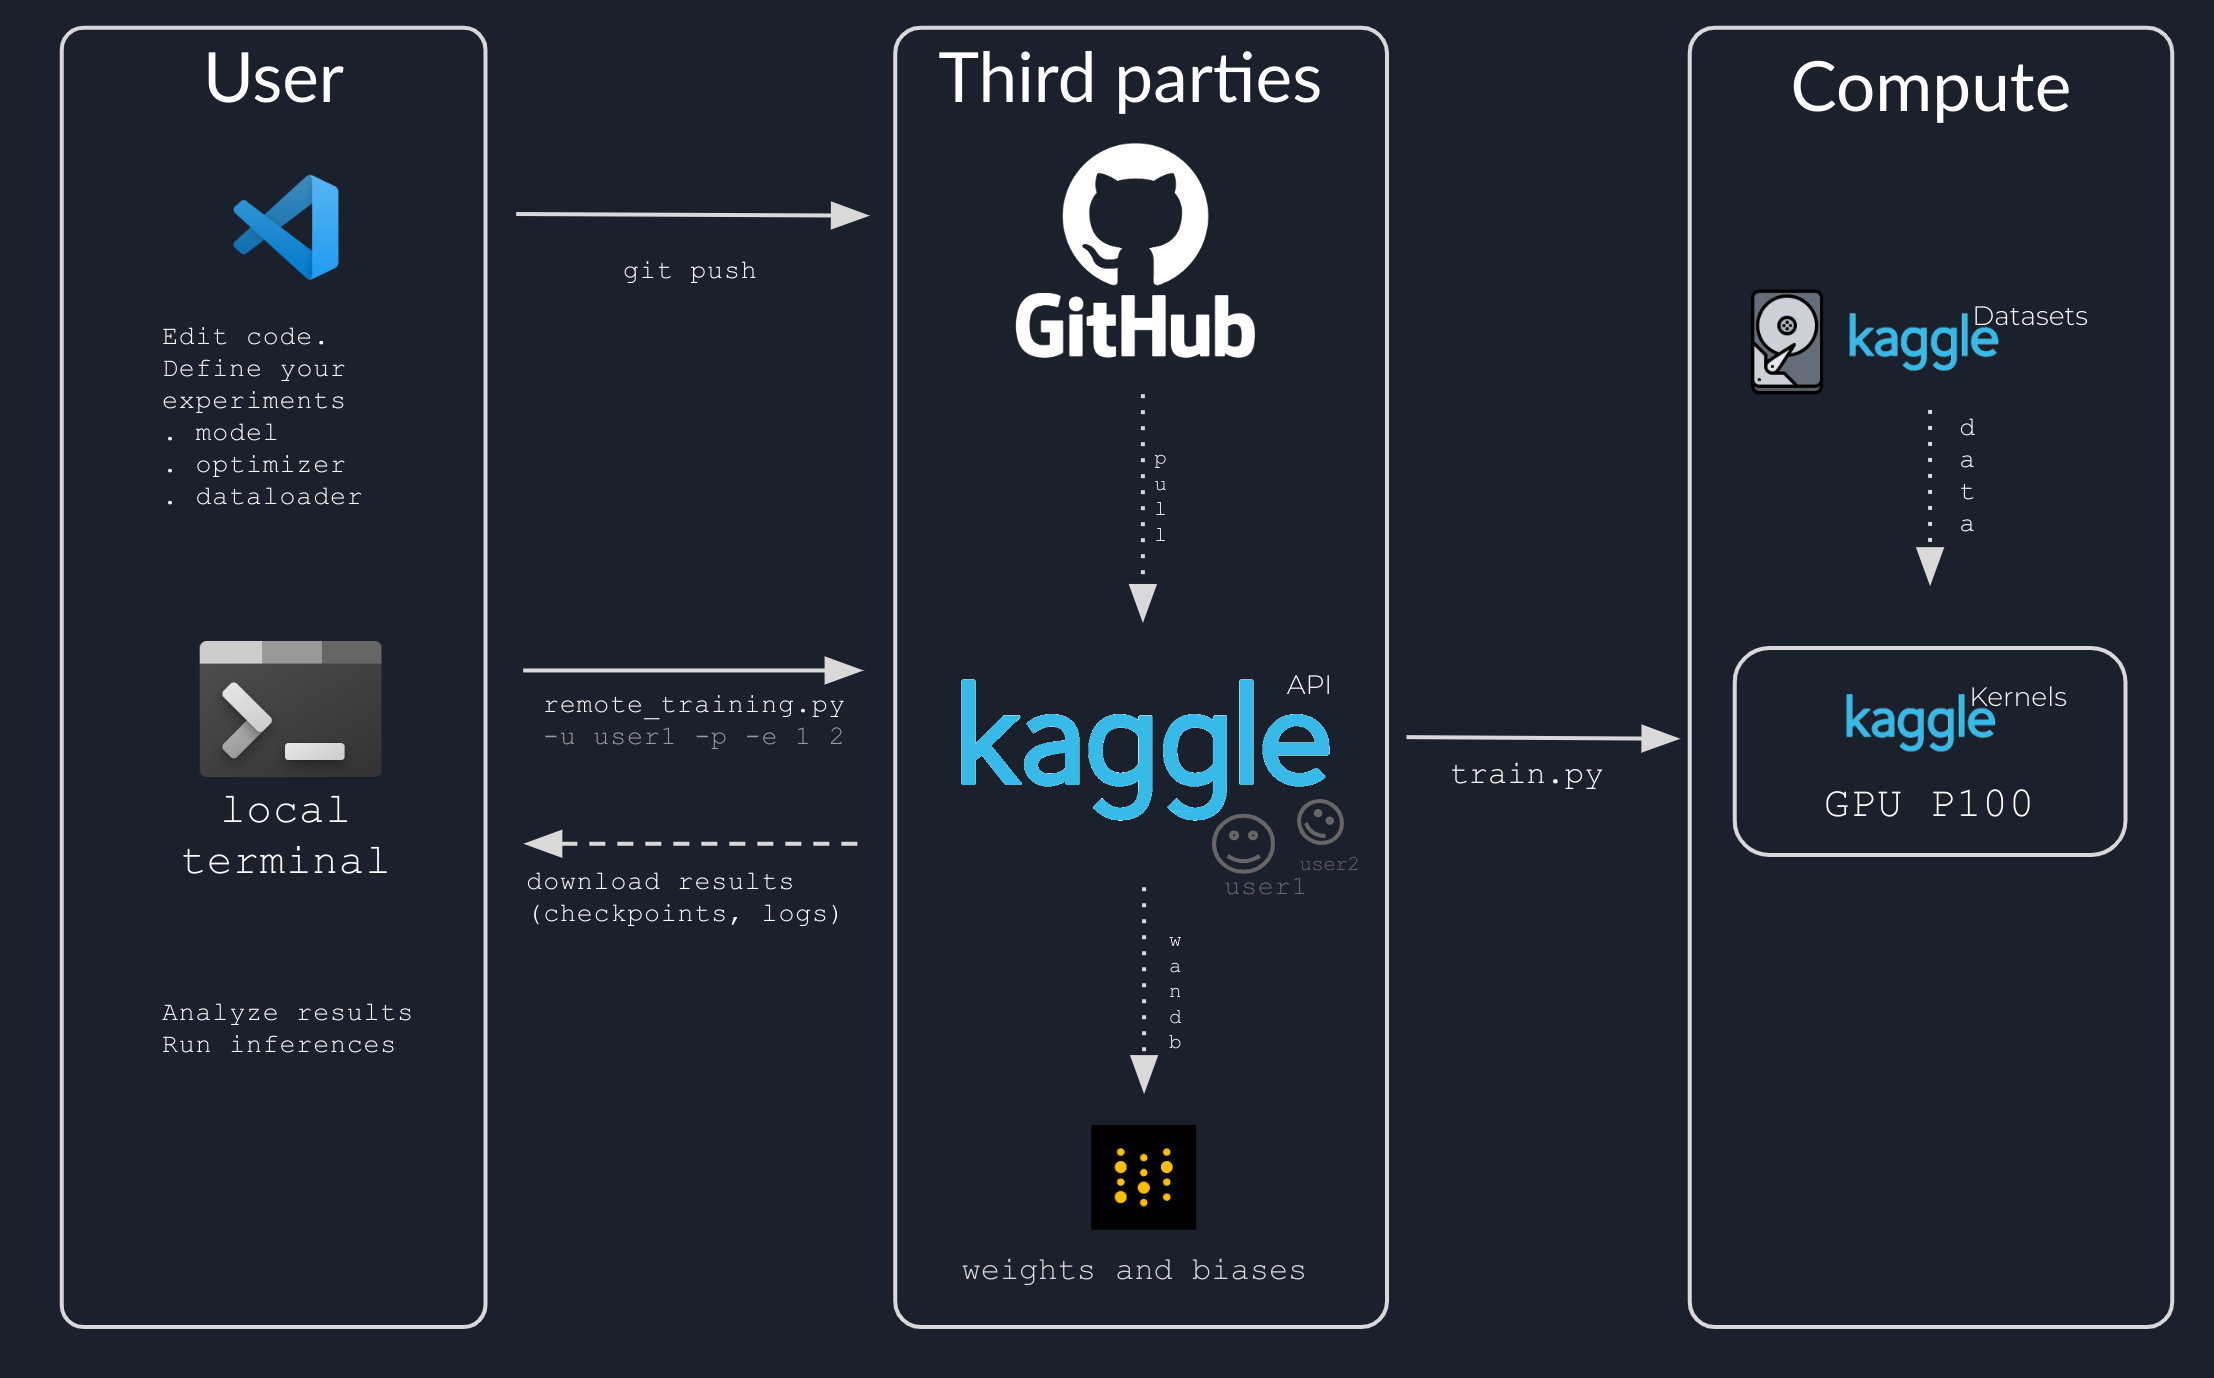
\includegraphics[width=0.5\textwidth]{figures/training_framework.png}
    \caption{Remote training framework allows accessing free GPU resources on Kaggle Kernels. Local code is synchronized through our \textbf{private Github repository} (until the 4th of February) so the remote notebook can be run with the same code. The \textbf{Kaggle dataset} feature is used to store the raw dataset and the preprocessed data (for each tokenizer, we have stored the preprocessed dataset which saves nearly 10 minutes of computation time at the begining of each experiment). To fine tune our own models, we use \href{https://huggingface.co/balthou}{Hugging Face} as an exchange platform so we could easily start from a checkpoint from any remove computer. The \textbf{Weights and biases} platform is used to track the experiments results and monitor the training. Once finished, trained models can be retrieved by pulling the results.
    Note that the small piece of code to help access Kaggle notebooks freely from the terminal was made available \href{https://github.com/balthazarneveu/mva\_pepites}{publicly} (totally independantly from this challenge) to be later used on other projects.
    }
    \label{fig:training_framework_schema}
\end{figure}

\subsection*{Training conditions}
\label{sec:training conditions}

\begin{table*}[ht]
    \centering
    \begin{tabular}{lcccc}
    \hline
    \textbf{Feature} & \textbf{Nvidia T500} & \textbf{Nvidia RTX 2060} & \textbf{Nvidia K100} & \textbf{Nvidia A4000} \\ \hline
    OS & Linux & Linux WSL & Linux in Docker & Linux \\  
    Location            & local laptop           & local laptop  & Kaggle  & Ecole Polytechnique  \\
    Access & direct & direct & Kaggle Kernels & SSH \\
    Dataset access & local SSD & local SSD & Kaggle dataset & remote download + SSD drives\\ 
    Memory           & 4 GB                        & 6 GB                           & 16 GB                          & 24 GB                          \\
    Student cost & - & Electricity $\approx$ +20 euros/month & Free & Free \\
    Availability & $\infty$ & $\infty$ & 30 hours/week 12hours/experiment & $\approx \infty$ weekends and night \\
    \hline
    \end{tabular}
    \caption{Comparison of the training platform and GPUs which were used during training}
    \label{table:gpu_comparison}
\end{table*}


To setup the training loop, we started on a single NVIDIA GeForce RTX T500 local GPU with 4Gb of RAM (\textit{the baseline provided by the challenge organizers did not even run because of memory limitation}). This was enough to make sure we could train, track and monitor progress of all our experiments and build a whole local training framework. We started by freezing the LLM weights to reduce the amount of memory required and get decent batch sizes even on the tiny T500 GPU. Due to low performances, the need to access bigger computation resources quickly came so we had to overcome this difficulty by making our framework agnostic to the training platform and still be able to recover our results and monitor from anywhere. The diversity of training and hardware platforms is shown in \ref*{table:gpu_comparison}. We considered using Google Colab Pro (datasets and models shared through Google drive) but with the consideration that we have long training times, the cost would have been prohibitive. We found a good compromise and did many experiments using Kaggle Kernels through the API which are free and provide GPU access with 16Gb of RAM during a maximum time of 12 hours per session and up to 30hours per week.
  \clearpage
\section{Appendix: State of the art}
\label{sec:sota_long_version}
In this supplementary section, we describe relevant works related to contrastive learning, graphs neural networks and the language models we've used.

% \subsubsection{Machine learning on molecules and text}
% \label{sec:sota_molec}
% Text-2-Mol \cite{text2mol} uses a language model jointly with a 3-layer GCN to create coherent representations among the two modalities.
% They introduce an interesting way to improve explainability: 

\subsubsection{Contrastive learning}
\label{sec:clip}
The CLIP \cite{CLIP} paper introduced by OpenAI builds image representation embedded in the same vector space as textual representations. This is a multi modality contrastive learning task, CLIP seems to rely on the fact that contrastive learning requires very large batch sizes (32000 image/text pairs per batch according to the authors) and that augmentations are mandatory.

Mol-CLR \cite{molCLR} tackles the problem of learning powerful representations solely from molecules only. Recent papers (such as SIMCLR\cite{SIMCLR}, Sim-SIAM \cite{simSIAM} and DINO\cite{DINO}) showed that great properties emerged from contrastive learning on images when applied to downstream tasks. So what about molecules? To be able to perform contrastive learning on a single modality, one needs to be able to augment the same data sample in several ways so that a human could still tell they're alike (in images, performing various crops or color transforms will still allow to recognize that the two augmented versions depict the same object for instance). MolCLR introduced interesting ways for molecule augmentations:

\textit{atom masking}: vector representation set to a fixed token so the atom is considered masked / undefined)

\textit{bound deletion}: removed a certain amount of edges across the graphs

\textit{subgraph removal}: mask an atom and it k-hop neighbors until it saturates to a certain amount of masked atoms (and finally remove the bounds inside the selected sub graph)

This technique could be thought as a pre-training task for the GCN although it seems to require a huge amount of data as the authors using approximately 10 millions of unique unlabelled molecules.

% \color{red}TODO - State of the art - Text2mol, CLIP, MolICLR augmentations=Contrastive learning for molecules only\color{black}



\subsubsection{BERT: a versatile language model}
\label{sec:bert}
The BERT paper \cite{bert} tackles the masked language modeling problem by training the encoder part of the Transformer \cite{transformer} model. BERT is a general purpose language representation model which become useful after fine tuning on downstream tasks (such as text classification or sentiment analyzis but not chatbots).  On the contrary to causal language modeling, BERT is not trained using next word prediction (unlike the GPT family) but instead uses the whole sentence to predict a masked word in the middle of it. BERT is able to build great language understanding capabilities which is what we're looking for here: a downstream task in the chemistry domain.
Researchers at Hugging Face \cite{distilbert} worked on a distilled version of BERT which results in smaller model with nearly as good language modeling capabilities (\textit{97\% as good, 60\% of the original size, 60\% faster}). Student model (DistilBERT) is trained to mimic the teacher (BERT)'s probability distribution for each output word. This is different from the original masked language training which supervises the network by telling if the predicted word matches with the ground truth word.
Sci-BERT\cite{scibert} is a BERT architecture which has been trained on a large scientific corpus made of more than one million scientific papers for a total of more than 3 billions of tokens (similar to BERT) and where the corpus has been tokenized. The tokenizer named SciVocab is provided along with the models on \href{https://huggingface.co/allenai/scibert_scivocab_uncased}{Hugging Face}.

\subsubsection{GCN: graph convolution networks}
\label{sec:GCN}

The pioneering and popular work of Kipf and Welling \cite{kipfwellinggcn} has defined a simple yet powerful local graph convolution operation which becomes extremely useful when stacked in a neural network architecture. To each input node of the graph, we attach a vector. Each node vector is processed using linear projection layers followed by non linearity function (such as ReLu), just like a MLP would process each nod vector separately. The graph structure is then exploited by averaging local neighbor node content (\textit{message passing}). Stacking several such operations allows extracting relevant graph structures. The processed graph output can either be used to classify each individual node (for nodes classification) or treating the graph as a whole by using an extra pooling layer (graph classification). For the molecules, we don't need to use the representation of each atom separately so a pooling mechanism will be used. We heavily rely on the \href{https://pytorch-geometric.readthedocs.io/en/latest/generated/torch_geometric.nn.conv.GCNConv.html}{Pytorch geometry GCNConv operator} which is the combination of a linear layer (mix channels) and the aggregation layer (average neighboring nodes). The symmetrically normalized adjacency matrix is used and allows numerical stability (we have not faced any issue when stacking these layers). One important point though is that the mean operator used to aggregate neighboring content may break the "counting" capability. For example, \textit{assume we have (H,H, O,O) in a neighborhood of an atom, the result of the convolution will be the same as the one with (H, O) neighbors}). We may have to keep in mind that the local structure may have been included a bit in the vector content thanks to the Mol-2-Vec \cite{mol2vec} of each node... the previous counter example may not be not such a problem. Additionally, it seems like there's a recent line of research (GIN  \cite{gin_isomorphism} - graph isomorphism networks) which may be able to distinguish structures better - \textit{roughly speaking the average aggregation is replaced by a sum operator}.
% There may exist more relevant architectures dedicated to pure structure extraction -> GIN , using the sum?. Interesting read here https://wandb.ai/syllogismos/machine-learning-with-graphs/reports/18-Limitations-of-Graph-Neural-Networks--VmlldzozODUxMzQ
  
  \newpage


\end{document}